% !TEX TS-program = pdflatex
% !TEX encoding = UTF-8 Unicode

% This is a simple template for a LaTeX document using the "article" class.
% See "book", "report", "letter" for other types of document.

\documentclass[11pt]{article} % use larger type; default would be 10pt

\usepackage[utf8]{inputenc} % set input encoding (not needed with XeLaTeX)
\usepackage{caption}
\usepackage{subcaption}
\usepackage{pdflscape}
\usepackage{lscape} 
\usepackage{rotating}
\usepackage{longtable}
\usepackage{graphicx}
\usepackage{float}
%%% Examples of Article customizations
% These packages are optional, depending whether you want the features they provide.
% See the LaTeX Companion or other references for full information.

%%% PAGE DIMENSIONS
\usepackage{geometry} % to change the page dimensions
\geometry{a4paper} % or letterpaper (US) or a5paper or....
% \geometry{margin=2in} % for example, change the margins to 2 inches all round
% \geometry{landscape} % set up the page for landscape
%   read geometry.pdf for detailed page layout information

\usepackage{graphicx} % support the \includegraphics command and options

% \usepackage[parfill]{parskip} % Activate to begin paragraphs with an empty line rather than an indent

%%% PACKAGES
\usepackage{booktabs} % for much better looking tables
\usepackage{array} % for better arrays (eg matrices) in maths
\usepackage{paralist} % very flexible & customisable lists (eg. enumerate/itemize, etc.)
\usepackage{verbatim} % adds environment for commenting out blocks of text & for better verbatim
% These packages are all incorporated in the memoir class to one degree or another...
\setlength{\textwidth}{150mm}
\setlength{\textheight}{250mm}
\setlength{\oddsidemargin}{6mm}
\setlength{\evensidemargin}{28mm}
\setlength{\topmargin}{-15mm}
%%% HEADERS & FOOTERS
\usepackage{fancyhdr} % This should be set AFTER setting up the page geometry
\pagestyle{fancy} % options: empty , plain , fancy
\renewcommand{\headrulewidth}{0pt} % customise the layout...
\lhead{Simheuristics}\chead{}\rhead{PEC3}
\lfoot{}\cfoot{\thepage}\rfoot{}

%%% SECTION TITLE APPEARANCE
\usepackage{sectsty}
\allsectionsfont{\sffamily\mdseries\upshape} % (See the fntguide.pdf for font help)
% (This matches ConTeXt defaults)

%%% ToC (table of contents) APPEARANCE
\usepackage[nottoc,notlof,notlot]{tocbibind} % Put the bibliography in the ToC
\usepackage[titles,subfigure]{tocloft} % Alter the style of the Table of Contents
\renewcommand{\cftsecfont}{\rmfamily\mdseries\upshape}
\renewcommand{\cftsecpagefont}{\rmfamily\mdseries\upshape} % No bold!

%%% END Article customizations

%%% The "real" document content comes below...

\title{Simheuristics}
\author{Alvarez Estarlich, Mauro \\ Requero Martín, David \\ Serrano Gómez, Enrique}
%\date{} % Activate to display a given date or no date (if empty),
         % otherwise the current date is printed 

\begin{document}
\maketitle

\section{Resumen y Comentario}

\subsection{A simheuristic algorithm for solving the permutation flow shop problem with stochastic processing times (Juan, A. et. al. (2014))}

El Flow Shop Scheduling Problem (FSP) es un problema que busca, en la mayoría de planteamientos, reducir el tiempo de producción de un conjunto de máquinas que tienen asociados N trabajos a realizar. Una variación del FSP es el Permutation Flow Shop Scheduling Problem (PFSP) que busca encontrar, realizando permutaciones en el orden de los trabajos, reducir el tiempo requerido para completar las tareas. Por último, el objeto de trabajo del articulo se centra en la generalización del PFSP, el PFSP with Stochastic Times (PFSPST) que añade el uso de valores aleatorios a la hora de determinar el tiempo de procesado de cada trabajo.\\[0.2cm]
La literatura relacionada con la variante estocástica del PFSP no es muy extensa, pues la mayor parte de artículos se han centrado en la variante determinista del problema. Por ello, algoritmo propuesto en el articulo para resolver este problema se basa en aprovechar los avances hechos en el estudio de la variante determinista para poder aplicarlos a la variante estocástica.\\[0.2cm]
Concretamente, el algoritmo propuesto consta de las siguientes etapas:
\begin{enumerate}
\item Convertir el problema en la variante determinista (PFSP, sin tiempos aleatorios).
\item Obtener soluciones de calidad, utilizando algoritmos eficientes basados en el PFSP (e.g. Iterated Local Search).
\item Ejecutar una simulación con las soluciones obtenidas, para obtener una muestra de los “tiempos para completar los trabajos”.
\item Repetir los puntos 2-3 hasta que las condiciones de parada del algoritmo se cumplan (ya sea por tiempo o por calidad de la solución). 
\end{enumerate}

\textbf{Valoración}

Desde mi punto de vista lo más destacable seria:
\begin{itemize}
\item En primer lugar, la simplificación del problema de la variante estocástica en la variante determinista resulta una estrategia muy beneficiosa ya que como se afirma en el artículo, la solución del modelo determinista necesariamente estará dentro del espacio de soluciones del modelo estocástico. Además, trabajando con la variante determinista se puede sacar provecho de los mejores resultados obtenidos en otros estudios. 
\item En segundo lugar, el uso de simulaciones para obtener los diferentes “tiempos de finalización de tareas” aporta la ventaja de no depender del uso de distribuciones estándar a la hora de determinar los tiempos de ejecución de las diferentes tareas, pues estas pueden no seguir dichas distribuciones por lo que se pueden ir adaptando a medida que el algoritmo se ejecuta.
\end{itemize}

\subsection{A simheuristic algorithm for the Single-Period Stochastic Inventory-Routing Problem with stock-out(Juan, A. et. al. (2014))}

El problema de enrutamiento de inventarios (IRP) integra los problemas de gestión de inventarios por parte del vendedor (VMI) y enrutamiento de vehículos de distribución (VRP). Partiendo de un centro de distribución se ha de suministrar un producto a un conjunto de centros con un stock inicial y una demanda. El objetivo de es minimizar los costes de transporte, inventario y de rotura de stock. \\[0.2cm]
Una de las variables principales del problema, la demanda, se puede modelar tanto desde un enfoque determinista como estocástico, en este caso aportando un mayor nivel de realismo y complejidad. Para resolver el IRP se propone un algoritmo simheurístico que combina simulación y el uso de una heurística aleatorizada. Se emplea la simulación de Monte Carlo para estimar los costes de inventario y rotura de stocks asociados a distintos escenarios de cada centro. Los costes de transporte de cada escenario se calculan empleando la heurística CWS. Se elige el escenario con menores costes totales como escenario base y se proponen nuevos escenarios para cada centro dentro del tiempo de computación establecido, seleccionándose como mejor solución aquella con menores costos totales. Con la finalidad de que las contribuciones de costes de inventario y costes de transporte sean similares, han de tener un mismo orden de magnitud. De no ser así el problema se correspondería a CVRP en el caso de costes de transporte elevados o a una estrategia descentralizada si los costes de inventarios son elevados.\\[0.2cm]

\textbf{Valoración}\\[0.2cm]

En el artículo se expone de forma detallada la motivación y los antecedentes que originan el concepto e IRP. Se valoran las distintas variaciones del problema y se expone la importancia de la elección de modelos estocásticos frente a determinísticos. La introducción permite al lector comprehender la totalidad del articulo sin necesidad de un conocimiento profundo del problema en particular. Además, introduce la motivación de usar simulación de Monte Carlo en combinación con las heurísticas típicamente empleadas en la resolución de problemas VRP. \\[0.2cm]
Resulta destacable, frente a otros artículos, que se desarrolla con mayor nivel de detalle el contenido y las implicaciones de los trabajos previos, permitiendo valorar mejor el desarrollo propuesto dentro de su ámbito. Otro aspecto reseñable es el énfasis que han hecho los autores en destacar los valores numéricos, las premisas y otra información técnica necesaria para reproducir la parte experimental del trabajo. Ya se indica que en otros trabajos similares esta información no se aporta, siendo imposible establecer una comparación cuantitativa entre distintas soluciones. \\[0.2cm]
Por último se ha de indicar que todo lo anterior se consigue en una extensión optima lo que facilita su lectura y pone en valor una buena labor de síntesis. 

\clearpage

\subsection{A review of simheuristics: Extending metaheuristics to deal with stochastic combinatorial optimization problems (Juan, A. et. al. (2015))}

\textbf{Simheuristics como metodología de optimización de simulación}\\[0.2cm]
Hay 2 enfoques diferentes:

\begin{itemize}
\item \underline{Simulation-Optimization (SO)}:\\[0.2cm]
El proceso de optimización utiliza datos de salida del modelo de simulación, que evalúa el rendimiento de la solución dada. Esa solución consiste en una serie de decisiones, que son los datos de entrada del modelo de simulación. Basado en esta y pasadas evaluación, el proceso de optimización decide sobre un nuevo conjunto de datos de entrada. Este modelo de simulación actúa como una Evaluation Function (EF)  del proceso de optimización.
Alternativamente, varias soluciones pueden ser simuladas para construir un modelo alternativo (SCM) que puede resolverse utilizando técnicas de optimización clásicas en vez de simulación. La solución a este metamodelo es considerada como una solución aproximada al problema original.
\item \underline{Hybrid Simulation-Analytic (HSA)}:\\[0.2cm]
Un modelo HSA es cualquier programa estocástico con escenarios muestreados. La simulación HSA es para potenciar el modelo analítico (AME) o para generar parte de la solución (SG).
En AME, la simulación se usa para refinar los parámetros de un modelo analítico de un problema específico. Este método necesita menor número de iteraciones en la simulación que EF.
\end{itemize}

\textbf{Lógica detras de Simheuristics}\\[0.1cm]

Este algoritmo sirve para afrontar eficientemente problemas de optimización combinatoria (COPs) que contienen componentes estocásticos. \\[0.1cm]

Este enfoque asume que, en escenarios con incerteza moderada, soluciones de alta calidad para la versión determinista del COP, probablemente serán soluciones de alta calidad para su correspondiente versión estocástica.\\[0.1cm]

Dada una instancia COP estocástica, su contraparte determinista es considerada. Después un algoritmo basado en metaheurística es ejecutado para realizar una búsqueda eficiente dentro del espacio de soluciones asociado al COP. Este proceso tiene como objetivo encontrar un conjunto de soluciones factibles de alta calidad para el COP determinista.\\[0.1cm]

Solo soluciones ‘prometedoras’ son enviadas al componente de simulación, lo que permite controlar el esfuerzo computacional empleado por la simulación durante el proceso de búsqueda.\\[0.1cm]

Valores estimados por la simulación pueden ser usados para mantener una lista de las mejores soluciones para el problema estocástico. Esto puede retroalimentar el metaheurístico para que intensifique la exploración de áreas del espacio de soluciones prometedoras.\\

\textbf{Conclusión}\\[0.2cm]
En vez de un enfoque de caja negra, donde las evaluaciones son realizadas solo por la simulación, los Simheuristics integran estrechamente la optimización y la simulación mediante la incorporación de información específica del problema.\\[0.2cm]


\textbf{Valoración}\\[0.2cm]

El artículo tiene una estructura simple y acertada porque te hace una introducción a lo que son los simheuristics y además te aporta muchos ejemplos de aplicaciones de metaheurística y simulación en diversos ámbitos. Una vez ya has visto diferentes aplicaciones te explica la lógica detrás de una combinación más estrecha de la simulación y la metaheurística, y el potencial que tiene este enfoque en diferentes ámbitos que han sido tratados anteriormente en el artículo.\\[0.2cm]
El artículo no te abruma con muchísima información diferente, todo gravita a la simulación y la metaheurística lo que ayuda a no perderse y las explicaciones junto con los ejemplos ayudan a que el tema puede entenderse más fácilmente.\\[0.2cm]
Tiene una conclusión que ayuda a retener la idea del artículo y esta referenciado correctamente.


\subsection{Learnheuristics: hybridizing metaheuristics with machine learning for optimization with dynamic inputs (Calvet, L. et. al. (2017))}

Este artículo revisa la literatura existente relacionada con la combinación de metaheurísticos y métodos de Machine Learning (ML) y luego presenta el concepto de Learnheuristics.\\[0.2cm]

\textbf{Uso de ML para mejorar Metaheurísticos:}

\begin{itemize}
\item \textbf{Hibridaciones específicamente localizadas:} Donde ML se aplica en un proceso especifico.\\[0.2cm]
La puesta a punto de parámetros metaheurísticos es conocida por tener un efecto significativo en el rendimiento de algoritmos. Hay 3 enfoques/estrategias:
\begin{itemize}
\item Estrategias de control de parámetros.
\item Estrategias de puesta a punto de parámetros.
\item Estrategias de puesta a punto de parámetros en instancias específicas.
\end{itemize}
Respecto a la gestión de población, los autores intentan extraer información de soluciones que ya han visitado y la utilizan para crear nuevas soluciones para explorar espacios de búsqueda más prometedores.\\

\item \textbf{Hibridaciones globales:} ML tiene un efecto mayor en el diseño metaheurístico.\\[0.2cm]
Algorithm selection problem (ASP)  tiene como objetivo predecir que algoritmo, dentro de un conjunto de algoritmos, va a tener un mejor rendimiento. Una red neural implementando una selección de parámetros suavizada es entrenada para predecir el mejor algoritmo.\\[0.2cm]
Hyper heuristics pueden ser descritos como métodos de búsqueda o mecanismos de aprendizaje para seleccionar o generar heurísticos para soluciones problemas computacionales de búsqueda. 
\item \textbf{Utilizando metaheurísticos para mejorar ML}\\[0.2cm]
Classification, Metaheurísticos han sido principalmente aplicados para la selección de atributos, extracción de atributos y puesta a punto de parámetros.\\[0.2cm]
Regression, Aplicados al uso de ML relacionado con el entrenamiento de modelos de regresión compleja. \\[0.2cm]
Clustering, Algoritmos de evolución diferencial son aplicados a este tipo de problemas. 
\item \textbf{Marco de trabajo LearnHeuristic}\\[0.2cm]
Este tiene como objetivo resolver problemas de optimización combinatoria (COPs) en los cuales los datos de entrada del modelo no son fijos de antemano. En lugar de eso, estos datos pueden variar de manera predecible de acuerdo con el estado de la solución parcialmente construida en cada iteración del heurístico de construcción. \\[0.2cm]
El objetivo de este tipo de problemas es minimizar las funciones de coste en relación a ciertos límites. La característica novedosa es que los datos de entrada de la función objetivo y/o los límites pueden depender de la estructura de la solución, lo que hace que estos datos sean dinámicos a medida que la solución parcial evoluciona.
\end{itemize}

\textbf{Valoración}\\[0.2cm]

Del artículo me ha parecido que el orden en el que aborda cada apartado es correcto. Va a hablar de metaheurística y Machine Learning y primero explica que es cada cosa, luego hace una revisión de la combinación de estas y luego explica el trabajo que hacen ellos con LearnHeuristics.\\[0.2cm]
Además del orden, las referencias utilizadas son muy diversas y da la oportunidad de profundizar en todo lo que menciona.\\[0.2cm]
Como punto negativo hay que mencionar que el articulo puede ser un poco denso y que ciertas partes, como la revisión de artículos, podrían haberse esquematizado mejor para que la lectura fuera más clara y amena.

\clearpage

{\fontsize{50}{60}\selectfont Diseño y desarrollo de un algoritmo de busqueda randomizada y heuristica CWS con demanda y recogida aplicada al VRP}

\renewcommand{\labelenumi}{\arabic{enumi}}
 \begin{enumerate}
   \item) \textbf{Introducción}\\[0.2cm]
El problema del rutaje de vehiculos (VRP de sus siglas en inglés) se centra en la busqueda del mejor conjunto de rutas por las que guiar a una flota de vehiculos de mercancias cuyo deber es abastecer a los clientes. Pero el problema puede ser planteado con diferentes grados de complejidad en funcion de las restricciones y detalles que se quieran considerar con tal de asemejar el sistema cada vez mas al mundo real. Las principales restricciones que se aplican al VRP se basan en:
   \begin{itemize}
       \item El uso de vehiculos con una capacidad finita en cuanto al transporte de mercancias.
       \item Que los vehiculos no pueden visitar dos veces un mismo cliente en su ruta de reparto.
       \item La presencia de un almacen desde del que todos los vehiculos salen y al que deben volver tras el reparto.
   \end{itemize} 
El VRP tiene un gran interes tanto por los beneficios económicos que puede reportar, asi como por los beneficios ecológicos que se pueden deducir del mismo.\\

Para esta segunda revisión del algoritmo añadimos las siguientes restricciones basadas en la oferta y la demanda de cada nodo:
   \begin{itemize}
	\item Asignación determinista de oferta y demanda, en contraposición a la variante estocástica que asigna valores para oferta y demanda a partir de una distribución.
	\item La capacidad del vehiculo de reparto se divide entre la mercancía que debe repartir y la que recoge de los nodos y cuya suma no puede exceder la capacidad total del vehiculo.
	\item Mercancía para entregar y la que se recoge de los nodos, no se mezcla ni se reparte entre nodos.
   \end{itemize} 

   \item) \textbf{Revisión de la literatura}

Hemos revisado los siguientes artículos para afrontar el problema con garantías:
	\begin{enumerate}
		\item Juan, A., Faulin, J., Grasman, S.E., Rabe, M., and Figueira, G. (2015). A review of simheuristics: Extending metaheuristics to deal with stochastic combinatorial optimization problems
		
		En este artículo nos hablan de cómo se puede extender la metaheurística para hacer frente a problemas de optimización combinatoria. Basándose en soluciones a problemas deterministas, simulan estas soluciones y los resultados de la simulación permiten analizar si son soluciones para el problema estocástico. 
		Simular el determinismo puede dar respuestas a lo estocástico.
		
		\item Juan, A., Barrios, B., Vallada, E., Riera, D., and Jorba, J. (2014). A simheuristic algorithm for solving the permutation flow shop problem with stochastic processing times.
		
		Aquí nos hablan sobre el Flow Shop Scheduling Problem (FSP) su variación con permutaciones y la generalización con tiempos de trabajo estocásticos. Se basan en trabajos deterministas para trabajar la parte estocástica.
		
		\item Juan, A., Grasman, S., Caceres, J., Bektas, T. (2014). A Simheuristic Algorithm for the Single-Period Stochastic Inventory Routing Problem with Stock-outs.
		
		Este artículo habla sobre el enrutamiento de inventarios (IRP) que integra la gestión de inventarios y enrutamiento de vehículos (VMI y VRP). Proponen un algoritmo simheurístico. Emplean la simulación de Monte Carlo para costes de inventario y heurística CWS para los costes de transporte.
		
		\item Calvet, L., De Armas, J., Masip, D., and Juan, A. (2017). Learnheuristics: hybridizing metaheuristics with machine learning for optimization with dynamic inputs.
		
		Por último, este articulo nos habla sobre las combinaciones que pueden hacerse entre metaheurísticos y ‘Machine Learning’ para la optimización de problemas. Además, presenta ‘LearnHeuristic’, que es una manera de trabajar que ayuda a resolver problemas de combinatoria mediante estas combinaciones.
\end{enumerate}

Estos artículos nos han permitido entender mejor el problema, aunque el artículo en el que nos hemos inspirado y nos ha ayudado más ha sido el articulo de Juan, A et. al. 2014 (3). Es semejante al VRPPD y además utiliza simulación de Monte Carlo y CWS con el que estábamos familiarizados al usarlo en la práctica anterior.


   \item) \textbf{Algoritmo desarrollado}\\[0.2cm]
A partir del algoritmo \textit{Clarke and Wright Savings} (CWS) hemos añadido el inicio sesgado como método para mejorar las soluciones y aportar variabilidad a los resultados.

El algoritmo básico tiene 3 fases:
\renewcommand{\labelenumii}{\arabic{enumii}}
	\begin{enumerate}
		\item Construir las aristas entre los nodos, calculando un coste asociado al movimiento entre nodos, este coste se usa como concepto de ahorro. Se genera una lista ordenada de las aristas que suponen mayor ahorro a menos ahorro.
		\item Construir una solución inicial con rutas desde el nodo inicial al nodo destino, solución que no es eficiente, pero es el punto de partida para ejecutar el siguiente paso.
		\item Se itera la lista de aristas creada y se comprueba si es factible fusionar las rutas que hay desde el nodo inicial a cada nodo en los extremos de la arista, teniendo en cuenta ademas, la capacidad del vehiculo para abastecer la demanda de los nodos y la necesidad de recoger mercancias de los nodos para llevarlos hasta el almacén. Al fusionar las rutas se consigue ahorrar costes y se empieza intentando fusionar las rutas mas costosas (que producen más ahorro).
	\end{enumerate}

Las principales diferencias con respecto al algoritmo presentado en la PEC anterior son:
\begin{enumerate}
\item Introduccion del parametro "pick-up" o "supply" que hace referencia al número de items que cada nodo tiene para ser recogido por el vehiculo de reparto.
\begin{figure}[H]
\centering
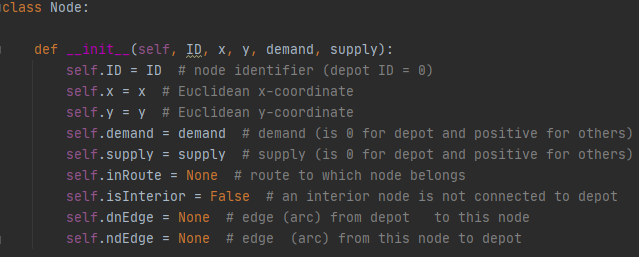
\includegraphics[width=\linewidth, height=6cm]{Node.png} 
\end{figure}
\item La opción de usar valores para la oferta y demanda generados de manera aleatoria en cada ejecución, siguiendo una dsitribucion definida por la media y la desviación estandar independientes. Para ello, seguimos las recomendaciones obtenidas de las conclusiones del trabajo de Ramaekers, K et. al. 2018, donde se analiza cual es la mejor forma de seleccionar una distribución a la hora de modelar la oferta/demanda. 
\begin{figure}[H]
\centering
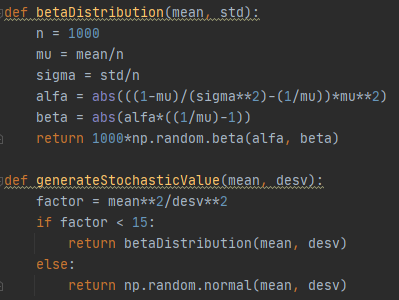
\includegraphics[width=0.55\linewidth, height=6cm]{StochDistrib.png} 
\end{figure}
\item Modificación de las condiciones necesarias para combinar dos rutas, teniendo en cuenta que ahora al visitar un nuevo nodo, se deberá tener en cuenta que se pueda satisfacer la demanda y tener espacio en el vehiculo para recoger los "supplies" del mismo.
\begin{figure}[H]
\centering
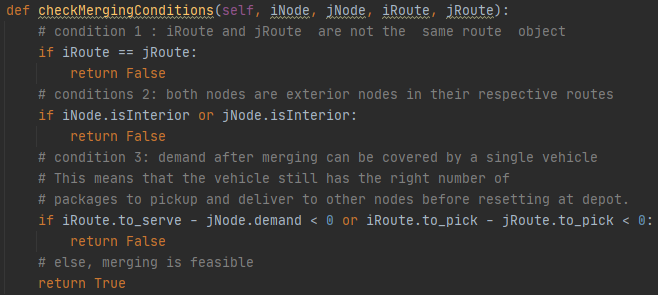
\includegraphics[width=\linewidth, height=6cm]{merge.png} 
\end{figure}
\end{enumerate}

   \item) \textbf{Experimento computacional y análisis de resultados}

Para la ejecución de los escenarios estocásticos se ha hecho uso de la librería lithops de Python. Dicha librería permite paralelizar la ejecución de funciones haciendo uso de servicios en la nube, en este caso concreto los backends de almacenamiento IBM Cloud Object Storage y de computación serverless IBM Cloud Functions.\\
En líneas generales su funcionamiento es análogo al módulo de multiprocessing de Python consiguiendo reducir de forma sustancial el tiempo de ejecución del programa incluso haciendo viables ciertas ejecuciones que en un PC convencional no serían viables. En el caso concreto de los backends de IBM se contempla su uso especifico para las aplicaciones de simulación de Monte Carlo y algoritmos genéticos. A pesar de las posibilidades que ofrece lithops, el elevado tamaño de las instancias limita la ejecución a de cada instancia 10 escenarios obtenidos de forma secuencial con 10 ejecuciones cada uno, obtenidas de forma paralela sobre el conjunto de instancias. \\[0.2cm]
Para el resto de los cálculos se ha empleado el módulo multiprocessing de Python con un procesador Intel Core i7 8750H con 6 núcleos y 12 hilos.\\[0.2cm]


	\resizebox{\textwidth}{!}{%
\begin{tabular}{lrrrrrrrrrrrr}
\toprule
 Instance &  Capacity &  Deterministic &  Stochast 1 &  Stochast 2 &  Stochast 3 &  Stochast 4 &  Stochast 5 &  Stochast 6 &  Stochast 7 &  Stochast 8 &  Stochast 9 &  Stochast 10 \\
\midrule
  Kelly01 &       550 &        7684.67 &       7788.49 &       7558.44 &       8075.98 &       7466.39 &       8090.22 &       7215.30 &       7490.09 &       7873.32 &       7584.11 &        7475.39 \\
  Kelly02 &       700 &       12832.82 &      12018.09 &      11496.08 &      11905.40 &      12121.63 &      11631.46 &      11799.74 &      11717.90 &      11769.51 &      12348.20 &       11815.40 \\
  Kelly03 &       900 &       17999.64 &      16657.35 &      17724.45 &      17369.22 &      17484.54 &      17131.32 &      16629.10 &      16928.87 &      16827.31 &      16526.58 &       16583.12 \\
  Kelly04 &      1000 &       24568.32 &      23388.88 &      22963.10 &      23065.68 &      22812.89 &      22922.13 &      23028.95 &      22852.53 &      23513.03 &      23250.35 &       23443.52 \\
  Kelly05 &       900 &       12028.70 &      12017.52 &      10938.33 &      12002.23 &      11735.23 &      12194.90 &      11762.61 &      11508.92 &      11796.83 &      11786.14 &       11570.85 \\
  Kelly06 &       900 &       15111.89 &      14565.06 &      13919.27 &      14271.66 &      14319.53 &      14518.98 &      13592.86 &      14070.63 &      13972.92 &      14250.17 &       14468.28 \\
  Kelly07 &       900 &       17755.14 &      16778.97 &      16174.20 &      16427.46 &      15792.96 &      16246.04 &      15980.06 &      15898.46 &      16770.05 &      16435.53 &       15986.65 \\
  Kelly08 &       900 &       19181.40 &      17428.92 &      18379.87 &      18303.92 &      17722.80 &      17864.38 &      17699.02 &      17422.82 &      16845.93 &      17366.72 &       18203.13 \\
  Kelly09 &      1000 &         860.03 &        732.87 &        772.01 &        780.37 &        750.17 &        809.48 &        749.34 &        750.06 &        755.84 &        738.56 &         799.26 \\
  Kelly10 &      1000 &        1055.21 &        976.83 &        993.54 &        959.12 &        946.75 &        909.13 &        976.66 &        912.34 &        965.07 &        986.04 &         921.24 \\
  Kelly11 &      1000 &        1271.10 &       1234.05 &       1159.63 &       1150.39 &       1135.97 &       1162.07 &       1176.52 &       1124.47 &       1086.94 &       1122.59 &        1158.15 \\
  Kelly12 &      1000 &        1476.76 &       1397.21 &       1395.32 &       1321.11 &       1376.15 &       1433.26 &       1358.76 &       1382.22 &       1366.81 &       1376.02 &        1439.75 \\
  Kelly13 &      1000 &         945.25 &        938.33 &        929.12 &        960.52 &        894.37 &        988.58 &        890.28 &        942.95 &        890.23 &        938.30 &         947.97 \\
  Kelly14 &      1000 &        1335.68 &       1125.36 &       1225.16 &       1210.27 &       1117.83 &       1192.68 &       1166.51 &       1179.34 &       1221.84 &       1252.89 &        1217.44 \\
  Kelly15 &      1000 &        1542.05 &       1477.59 &       1399.74 &       1435.03 &       1444.98 &       1463.37 &       1467.92 &       1523.48 &       1459.01 &       1429.63 &        1507.22 \\
  Kelly16 &      1000 &        1817.43 &       1726.75 &       1731.44 &       1806.69 &       1835.46 &       1762.15 &       1743.33 &       1804.95 &       1762.70 &       1772.10 &        1749.09 \\
  Kelly17 &       200 &         703.96 &        756.00 &        737.85 &        785.60 &        802.13 &        712.94 &        768.38 &        773.69 &        761.34 &        710.19 &         752.03 \\
  Kelly18 &       200 &         971.44 &       1002.57 &       1015.81 &       1062.53 &       1049.88 &       1046.82 &       1024.96 &       1063.88 &       1067.26 &       1062.26 &        1024.22 \\
  Kelly19 &       200 &        1262.29 &       1400.39 &       1418.92 &       1386.35 &       1294.52 &       1375.72 &       1389.26 &       1394.48 &       1358.69 &       1396.61 &        1397.30 \\
  Kelly20 &       200 &        1712.61 &       1755.78 &       1772.81 &       1752.89 &       1877.90 &       1822.62 &       1780.32 &       1794.92 &       1812.93 &       1685.27 &        1842.59 \\
\bottomrule
\end{tabular}}\\[0.2cm]

\resizebox{\textwidth}{!}{%
\begin{tabular}{lrrrrrrrrrrr}
\toprule
Instance &  Capacity &   gap1 &   gap2 &   gap3 &   gap4 &   gap5 &   gap6 &   gap7 &   gap8 &   gap9 &  gap10 \\
\midrule
  Kelly01 &       550 &   1.35 &  -1.64 &   5.09 &  -2.84 &   5.28 &  -6.11 &  -2.53 &   2.45 &  -1.31 &  -2.72 \\
  Kelly02 &       700 &  -6.35 & -10.42 &  -7.23 &  -5.54 &  -9.36 &  -8.05 &  -8.69 &  -8.29 &  -3.78 &  -7.93 \\
  Kelly03 &       900 &  -7.46 &  -1.53 &  -3.50 &  -2.86 &  -4.82 &  -7.61 &  -5.95 &  -6.51 &  -8.18 &  -7.87 \\
  Kelly04 &      1000 &  -4.80 &  -6.53 &  -6.12 &  -7.15 &  -6.70 &  -6.27 &  -6.98 &  -4.30 &  -5.36 &  -4.58 \\
  Kelly05 &       900 &  -0.09 &  -9.06 &  -0.22 &  -2.44 &   1.38 &  -2.21 &  -4.32 &  -1.93 &  -2.02 &  -3.81 \\
  Kelly06 &       900 &  -3.62 &  -7.89 &  -5.56 &  -5.24 &  -3.92 & -10.05 &  -6.89 &  -7.54 &  -5.70 &  -4.26 \\
  Kelly07 &       900 &  -5.50 &  -8.90 &  -7.48 & -11.05 &  -8.50 & -10.00 & -10.46 &  -5.55 &  -7.43 &  -9.96 \\
  Kelly08 &       900 &  -9.14 &  -4.18 &  -4.57 &  -7.60 &  -6.87 &  -7.73 &  -9.17 & -12.18 &  -9.46 &  -5.10 \\
  Kelly09 &      1000 & -14.79 & -10.23 &  -9.26 & -12.77 &  -5.88 & -12.87 & -12.79 & -12.11 & -14.12 &  -7.07 \\
  Kelly10 &      1000 &  -7.43 &  -5.84 &  -9.11 & -10.28 & -13.84 &  -7.44 & -13.54 &  -8.54 &  -6.55 & -12.70 \\
  Kelly11 &      1000 &  -2.91 &  -8.77 &  -9.50 & -10.63 &  -8.58 &  -7.44 & -11.54 & -14.49 & -11.68 &  -8.89 \\
  Kelly12 &      1000 &  -5.39 &  -5.51 & -10.54 &  -6.81 &  -2.95 &  -7.99 &  -6.40 &  -7.45 &  -6.82 &  -2.51 \\
  Kelly13 &      1000 &  -0.73 &  -1.71 &   1.62 &  -5.38 &   4.58 &  -5.81 &  -0.24 &  -5.82 &  -0.73 &   0.29 \\
  Kelly14 &      1000 & -15.75 &  -8.27 &  -9.39 & -16.31 & -10.71 & -12.67 & -11.70 &  -8.52 &  -6.20 &  -8.85 \\
  Kelly15 &      1000 &  -4.18 &  -9.23 &  -6.94 &  -6.30 &  -5.10 &  -4.81 &  -1.20 &  -5.39 &  -7.29 &  -2.26 \\
  Kelly16 &      1000 &  -4.99 &  -4.73 &  -0.59 &   0.99 &  -3.04 &  -4.08 &  -0.69 &  -3.01 &  -2.49 &  -3.76 \\
  Kelly17 &       200 &   7.39 &   4.81 &  11.60 &  13.95 &   1.28 &   9.15 &   9.91 &   8.15 &   0.89 &   6.83 \\
  Kelly18 &       200 &   3.20 &   4.57 &   9.38 &   8.07 &   7.76 &   5.51 &   9.52 &   9.86 &   9.35 &   5.43 \\
  Kelly19 &       200 &  10.94 &  12.41 &   9.83 &   2.55 &   8.99 &  10.06 &  10.47 &   7.64 &  10.64 &  10.70 \\
  Kelly20 &       200 &   2.52 &   3.51 &   2.35 &   9.65 &   6.42 &   3.95 &   4.81 &   5.86 &  -1.60 &   7.59 \\
\bottomrule
\end{tabular}}\\[0.2cm]

El resultado determinístico es aquel obtenido empleando demandas y ofertas en cada nodo cuyos valores eran fijos. Se ha establecido como caso ideal en el cual su comportamiento es plenamente predecible. Frente a este escenario se han simulado 10 escenarios estocásticos cuyos costes se han obtenido a partir de ofertas y demandas variables, obtenidas empleando las distribuciones anteriormente expuestas. En dichas simulaciones se ha empleado aleatorización sesgada con un parámetro $\beta$=0.5 para una distribución geométrica, lo que supone un comportamiento intermedio entre uno explorativo puro y uno explotativo puro. Los valores medios del conjunto de los escenarios estocásticos no resultan de gran utilidad ya que por la ley de los grandes números convergerán al caso determinístico, por lo que es experimento realizado solo busca la obtención de una muestra de hipotéticos escenarios.\\[0.2cm]
En general la mayoría de las instancias de Kelly1 a Kelly16 presentan menores costes que el caso determinístico en los casos observándose valores de gap negativos de hasta -15\%. De forma similar las instancias Kelly17 a Kelly 20 no presentan menores costes que el escenario determinístico. Puede estar causado, a parte de la distribución de los nodos en dichas instancias, al hecho de que los vehículos empleados en esos casos menor capacidad que los presentes en los otros casos , al menos, en cuanto a los niveles de demanda y oferta se refiere.  

   \item) \textbf{Conclusiones y trabajo futuro}\\[0.2cm]

A partir de los resultados obtenidos podemos concluir que:

\begin{itemize}
\item 
\end{itemize}

Como trabajo futuro proponemos: 

\begin{itemize}
\item Analizar si con distintas funciones de coste (o savings) se generan mejores resultados.
\item Estudiar si con un mayor numero de iteraciones, se mejoran de manera significativa los resultados obtenidos y en que punto las soluciones dejan de mejorar.
\item Explorar para diferentes valores de $\beta$ entre 0.4 y 0.6, si las soluciones mejoran.
\item Aplicar diferentes métodos de splitting en función de la topología de la red.
\item Determinar que areas de la ejecución pueden ser paralelizadas para mejorar el rendimiento de la ejecución del algoritmo.
\end{itemize}

 \end{enumerate}

\pagestyle{empty}
\begin{landscape}

\end{landscape}
\pagestyle{plain}

\end{document}
